\documentclass[a4paper]{article}
\usepackage[12pt]{extsizes}
\usepackage[utf8]{inputenc}
\usepackage[T2A]{fontenc}
\usepackage{amssymb,amsmath,mathtext}
\usepackage{indentfirst,amsfonts}
\usepackage[english, russian]{babel}
\usepackage{setspace,amsmath}
\usepackage{graphicx}
\usepackage[left=30mm, top=20mm, right=10mm, bottom=20mm, nohead, footskip=10mm]{geometry} % настройки полей документа

\graphicspath{{graphs/}}

\begin{document}
	\begin{titlepage} % начало документа
		
		% НАЧАЛО ТИТУЛЬНОГО ЛИСТА
		\begin{center}
			\footnotesize{ФЕДЕРАЛЬНОЕ ГОСУДАРСТВЕННОЕ БЮДЖЕТНОЕ ОБРАЗОВАТЕЛЬНОЕ }\\ 
			\footnotesize{УЧРЕЖДЕНИЕ ВЫСШЕГО ОБРАЗОВАНИЯ}\\
			\small{«МОСКОВСКИЙ ГОСУДАРСТВЕННЫЙ УНИВЕРСИТЕТ}\\
			\small{имени М.В.ЛОМОНОСОВА»}\\
			\hfill \break
			\normalsize{ФИЗИЧЕСКИЙ ФАКУЛЬТЕТ}\\
			\hfill \break
			\normalsize{КАФЕДРА МАТЕМАТИЧЕСКОГО МОДЕЛИРОВАНИЯ И ИНФОРМАТИКИ}\\
			\hfill \break
			\hfill \break
			\hfill \break
			\hfill \break
			\hfill \break
			\hfill \break
			\large{\textbf{Нейросетевой синтез текстур с трендами}}\\
		\end{center}
		
		\hfill \break
		
		\begin{flushright}
			Выполнил студент \\
			\hfill \break
			435 группы:\\
			\hfill \break
			Будакян Я. С.\\
			\hfill \break
			\hfill \break
			\hfill \break
			Научный руководитель: \\
			\hfill \break
			к.т.н., доц. Грачев Е. А.\\
			\hfill \break
		\end{flushright}
		
		\hfill \break
		\hfill \break
		\hfill \break
		\hfill \break
		\hfill \break
		\hfill \break
		
		\begin{center}
			Москва \\
			\hfill \break
			2017 
		\end{center}
		
		\thispagestyle{empty} % выключаем отображение номера для этой страницы
		
		% КОНЕЦ ТИТУЛЬНОГО ЛИСТА
		
	\end{titlepage}  % КОНЕЦ ДОКУМЕНТА !
	%учитываем титульный лист в нумерации
	\setcounter{page}{2}
	\section{Введение}
		Цель работы состоит в построении процедуры синтеза изображений среды, которые будут содержать в себе тренд. Под текстурой с трендом понимается изображение, в котором есть изменение некоторой статистической характеристики вдоль одного из направлений. Такими характеристиками, например, могут быть изменение интенсивности появления частиц среды или изменение пористости среды. \\
		\begin{figure}[h]
			\centering{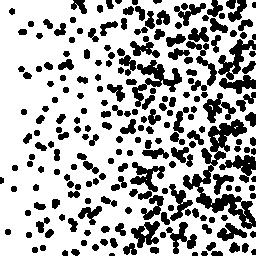
\includegraphics[width=0.35\linewidth]{trend-sample}}
			\caption{Пример текстуры с трендом интенсивности частиц.}
			\label{trend-example}
		\end{figure}
	\section{Математическая постановка}
		Рассмотрим многомерное пространство $X$, содержащее множество всех изображений $x$: $X = \{x\}$. Тогда обучающая выборка изображений с трендами $D = \{x_i\}$ задает в этом пространстве вероятностное распределение $P_X : X \longrightarrow [0,1]$, устроенное таким образом, что точки, соответствующие изображениям из выборки, имеют высокую вероятность, а остальные - низкую. Это так называемая вероятностная постановка задачи обучения \cite{Voron-ML, GAN}. Тогда с математической точки зрения задача синтеза текстуры с трендом сводится к синтезу случайного изображения $x'$, принадлежащего распределению, близкому к задаваемому обучающей выборкой:
		$$ P_{X'} \approx P_X, \quad x' \sim X'$$
		Для упрощения задачи, сузим множество изображений с трендами до множества изображений, удовлетворяющих следующим ограничениям:
		\begin{itemize}
			\item Это монохромные изображения 256 x 256 пикселей
			\item Изменяющимся свойством является интенсивность появления частиц $\lambda$
			\item Тренд является линейным и направлен вдоль оси изображения $z_1$: 
			$ \lambda = \lambda_0 + k z_1 $
		\end{itemize}
	\section{Существующие подходы к синтезу}
		Есть несколько подходов к решению задачи подобного рода:
		\begin{itemize}
			\item 'Классический' статистический подход
			\item Базовый нейросетевой подход
			\item Генеративные состязательные сети (Generative Adversarial Networks - GAN)
		\end{itemize}
		\subsection{'Классический' статистический подход}
			\begin{itemize}
				\item Вводится параметризированное семейство распределений вероятности $P_{\theta}(x)$
				\item Параметры $\theta$ находятся из обучающей выборки:
				$$ \mathcal{L}_{\theta}(D) = \prod_{x \in D} P_{\theta}(x) $$
				$$ \theta^{*} = \underset{\theta}{\arg\max} \mathcal{L}_{\theta}(D)$$
				\item Генерируется объект(изображение) из распределения $ P_{\theta^{*}}$
			\end{itemize}
			Этот подход приводит к проблемам:
			\begin{itemize}
				\item Пространство параметров $\theta$ может быть огромной размерности
				\item Известной параметрической модели распределения может вообще не существовать
			\end{itemize}
			Простой пример - синтез человеческих лиц: с помощью классического подхода эта задача не была решена с хорошим качеством.
		\subsection{Базовый нейросетевой подход}
			\begin{itemize}
				\item Вводится параметризированное семейство распределений вероятности $P_{\theta}(x)$
				\begin{itemize}
					\item Вводятся скрытые переменные $V$ и функция(нейросеть) для получения $x$ из $V$ (фактически, классификация, развернутая в другую сторону)
				\end{itemize}
				\item Определяются параметры распределения (т.е. обучение нейросети)
				\item Генерируется объект(изображение) из $ P_{\theta^{*}}$
			\end{itemize}
			Этот подход возможен, однако на практике трудноосуществим или не приводит к хорошему качеству генерации \cite{GAN-2}.
		\subsection{GAN - генеративные состязательные сети}
			Архитектура GAN была придумана в 2014 году специально для решения задачи генерации объектов из сложных распределений. \\
			Переформулируем изначальную задачу нахождения такой процеруды генерирования $X'$, чтобы $ P_{X'} \approx P_X$:
			$$ \rho(P_{X'}, P_X) \longrightarrow \underset{P_{X'}}{\min} $$
			Введем параметризированную процедуру генерации:
			$$ X' = g_{\theta}(\cdot) $$
			Переформулируем:
			$$ \rho(P_{X'}, P_X) \longrightarrow \underset{P_{X'}}{\min} $$
			$$ \rho(g_{\theta}(\cdot), P_X) \longrightarrow \underset{g_{\theta}(\cdot)}{\min} $$
			$$ \rho(g_{\theta}(V), P_X) \longrightarrow \underset{\theta}{\min} $$
			Возникает вопрос: что использовать в качестве метрики похожести двух распределений $\rho$, где одно из распределений задано обучающей выборкой.
			В качестве такой метрики можно использовать функцию потерь обученного классификатора, потому что естественно предположить, что чем чаще ошибается обученный классификатор, тем больше одно распределение похоже на другое. Тогда задача примет вид:
			$$ \rho(P_{X'}, P_X) \longrightarrow \min \Leftrightarrow L \longrightarrow \max, $$
			где $L$ - функция потерь обученного классификатора.
			Соответственно, можно ввести две нейросети:
			\begin{itemize}
				\item $d_{\zeta}(x)$ - классификатор для измерения расстояния, \textbf{'дискриминатор'}
				\item $g_{\theta}(x)$ - сеть, трансформирующая шум в $X'$, \textbf{'генератор'}
			\end{itemize}
			Суть использования двух сетей состоит в том, что они обучаются совместно, конкурируя друг с другом: генератор пытается имитировать целевое распределение, а дискриминатор пытается классифицировать поступающие от генератора и из обучающей выборки изображения на 2 класса: реальные (из изначального распределения $P_X$) и ложные (из $P_{X'}$, т.е. произведенные генератором).
			Для дальнейшего рассмотрения введем функцию потерь дискриминатора(например, logloss):
			$$ l_1 = l(d_{\zeta}(x), 1) \text{ - ошибка 1 рода} $$
			$$ l_2 = l(d_{\zeta}(x'), 0) \text{ - ошибка 2 рода}$$
			$$ L(X, X') = \frac{1}{2} \mathbb{E}_{X} l_1 + \frac{1}{2} \mathbb{E}_{X'} l_2 = -\frac{1}{2} (\mathbb{E}_{X} \log d_{\zeta}(x) + \mathbb{E}_{X'} \log (1 - d_{\zeta}(x'))) = $$
			$$ =  -\frac{1}{2} (\mathbb{E}_{X} \log d_{\zeta}(x) + \mathbb{E}_{V} \log (1 - d_{\zeta}(g_{\theta}(v)))) = L(\zeta, \theta) .$$
			Функция потерь обученного классификатора:
			$$ L^*(\theta) = \underset{\zeta}{\min} L(\zeta, \theta) $$
			Соответственно,
			$$ \underset{\zeta}{\min} L(\zeta, \theta) \longrightarrow \underset{\theta}{\max} $$
			$$ \theta^* = \underset{\theta}{\arg\max} \left[ \underset{\zeta}{\min} L(\zeta, \theta) \right] $$
			Определим оптимальный дискриминатор:
			$$ d^*_{\theta} = d_{\zeta^*(\theta)} $$
			$$ \zeta^*(\theta) =  \underset{\zeta}{\arg\min} L(\zeta, \theta)$$
	\section{Обучение GAN}
		Итак, задача обучения GAN свелась к нахождению
		$$ \theta^* = \underset{\theta}{\arg\max} \left[ \underset{\zeta}{\min} L(\zeta, \theta) \right] $$
		Решить ее можно, например, методом стохастического градиентного спуска:
		$$ \Delta \theta \sim \nabla L(\zeta^*(\theta), \theta)$$
		Для малых изменений $\Delta \theta$:
		$$ \nabla L(\zeta^*(\theta), \theta) \approx \nabla L(\zeta^*(\theta), \theta + \Delta \theta) $$
		В итоге, процесс обучения принимает следующий вид:
		\begin{itemize}
				\item Обучаем дискриминатор при фиксированном генераторе
				\item Обучаем генератор при фиксированном дискриминаторе
				\item Повторяем до сходимости параметров обеих моделей
		\end{itemize}
		\begin{figure}
			\centering{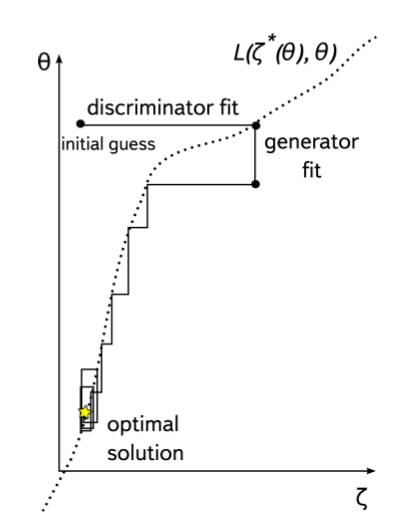
\includegraphics[width=0.4\linewidth]{gan-training}}
			\caption{Схематическое изображение процесса обучения GAN.}
			\label{gan-train}
		\end{figure}
	\section{pix2pix GAN}
		Для решения задачи было попробовано применить модификацию GAN-сети под названием "pix2pix GAN" \cite{p2p}. Ее отличие от схемы GAN, введенной выше, состоит в том, что вместо шума на вход генератору приходят другие изображения, на которых он основывается при синтезе. Схематически ее устройство изображено на (Рис. \ref{p2p}).
		\begin{figure}
			\centering{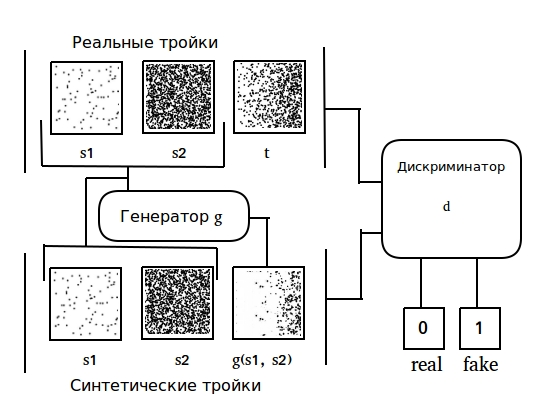
\includegraphics[width=0.65\linewidth]{p2p}}
			\caption{Схематическое устройство сети pix2pix GAN.}
			\label{p2p}
		\end{figure}
		Для pix2pix сети общий функционал потерь выглядит следующим образом: $$ L(G, D) = L_{adv}(G, D) + \eta \mathbb{E}_{p_{data}(s_1, s_2, r)} (\parallel r - G(s_1, s_2) \parallel_1)$$
		$$ L_{adv}(G, D) = \mathbb{E}_{p_{data}(s_1, s_2, r)}\log D(s_1, s_2, r) +  \mathbb{E}_{p_{data}(s_1, s_2)} \log (1 - D(s_1, s_2, G(s_1, s_2)))$$
		где G, D - генератор и дискриминатор, $(s_1, s_2, r)$ - тройка изображений (интенсивность слева, справа и реальное изображение с трендом),  $\mathbb{E}_{p_{data}(s_1, s_2, r)}$ - мат. ожидание логарифмического правдоподобия того, что тройка изображений $(s_1, s_2, r)$ принадлежит вероятностному распределению реальных троек $p_{data}(s_1, s_2, r)$, а $p_{data}(s_1, s_2)$ соответствует распределению реальных изображений $s_1, s_2$.
		\begin{figure}
			\centering{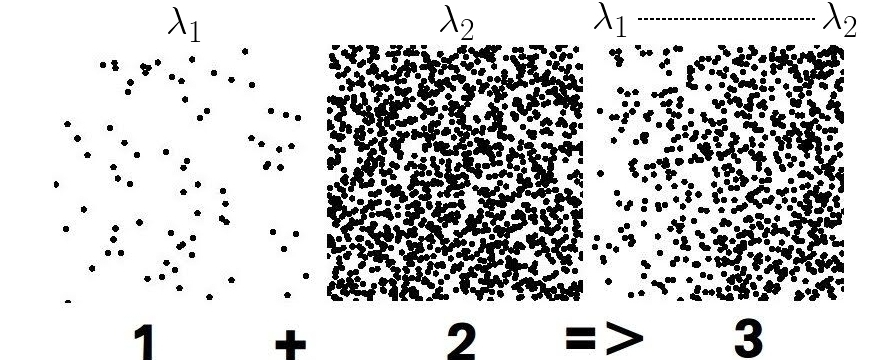
\includegraphics[width=0.75\linewidth]{p2p-gen}}
			\caption{Вход и желаемый выход нейросети-генератора.}
			\label{p2p-gen}
		\end{figure}
		\begin{figure}
			\centering{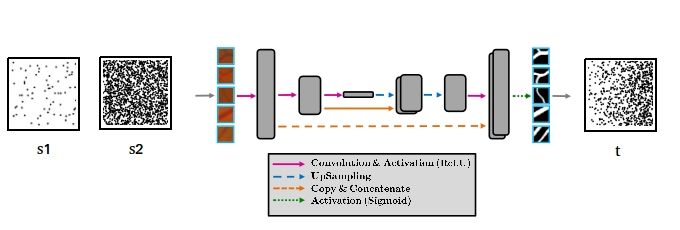
\includegraphics[width=1\linewidth]{unet-scheme}}
			\caption{Схематическое изображение нейросети-генератора.}
			\label{unet-sheme}
		\end{figure}
	\section{Критерий качества}
		После обучения генератора, необходимо проверить, что сгенерированные им изображения действительно имеют искомые характеристики. Для этого нужно ввести специальную метрику, которая будет учитывать наличие в изображении тренда интенсивности частиц. Было решено использовать среднюю плотность черных пикселей в некотором окне, и проходить этим окном по изображению (Рис. \ref{window}):
		\newpage
		$$\xi_k = \frac{1}{H w}{\sum_{i=k}^{k+w} \sum_{j=0}^{H}\left| \frac{x(i, j) - 255}{255} \right|}, $$$$k = \overline{1, W - w + 1} $$
		\begin{figure}
			\centering{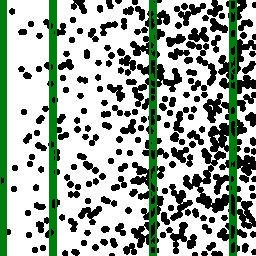
\includegraphics[width=0.35\linewidth]{metrics}}
			\caption{Прохождение окном, W, H - размеры изображения, w - ширина окна.}
			\label{window}
		\end{figure}
		\\
		Построив график $\xi(k)$, можно увидеть, как меняется плотность пикселей и прослеживается ли тренд. В качестве метрики можно взять среднеквадратичную ошибку:
		$$ \xi = \frac{1}{W-w}\sum_{k=1}^{W-w+1} (\xi_k - \xi_{0k})^2,$$
		где $\xi_{0k}$ - это $\xi_k$, усредненное по примерам из обучающей выборки. Соответственно, чем меньше значение метрики, тем лучше тренд, присутствующий на сгенерированном изображении, приближает искомый.
	\section{Результаты}
		Было проведено обучение нейросети описанной архитектуры при различных гиперпараметрах (в частности, количестве фильтров на первом сверточном слое). Обучающей выборкой был массив из 3500 троек изображений. Примеры сгенерированных текстур приведены на (Рис. \ref{generated}).
		\begin{figure}
			\begin{minipage}{0.3\linewidth}
				\centering{
\includegraphics[width=0.75\linewidth]{nf8} \\ nf8}
			\end{minipage}
			\hfill
			\begin{minipage}{0.3\linewidth}
				\centering{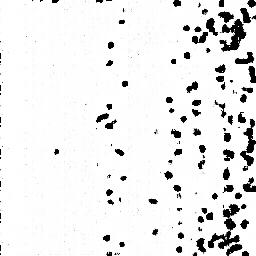
\includegraphics[width=0.75\linewidth]{nf16} \\ nf16}
			\end{minipage}
			\hfill
			\begin{minipage}{0.3\linewidth}
				\centering{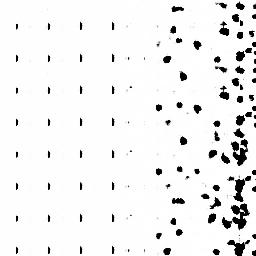
\includegraphics[width=0.75\linewidth]{nf16_woUnet} \\ nf16-woUnet}
			\end{minipage}
			\hfill
			\begin{minipage}{0.3\linewidth}
				\centering{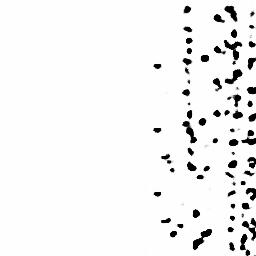
\includegraphics[width=0.75\linewidth]{nf16_3x3_woUnet} \\ nf16-3x3-woUnet}
			\end{minipage}
			\hfill
			\begin{minipage}{0.3\linewidth}
				\centering{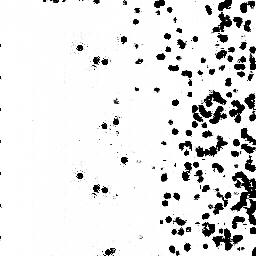
\includegraphics[width=0.75\linewidth]{nf32} \\ nf32}
			\end{minipage}
			\hfill
			\begin{minipage}{0.3\linewidth}
				\centering{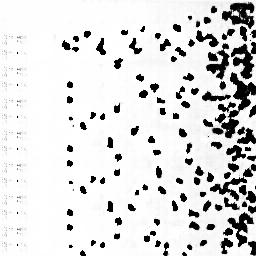
\includegraphics[width=0.75\linewidth]{nf32_woUnet} \\ nf32-woUnet}
			\end{minipage}
			\caption{Примеры сгенерированных текстур.}
			\label{generated}
		\end{figure}
		Была подсчитана введенная метрика для сгенерированных наборов текстур. Графики плотности черных пикселей в зависимости от сдвига окна, квадратичного отклонения от тренда и сами значения метрики приведены на (Рис. \ref{tr-1}, \ref{tr-2}, \ref{err1}, \ref{err2}) и в (Таб. \ref{table1}, \ref{table2})
		\begin{figure}
			\centering{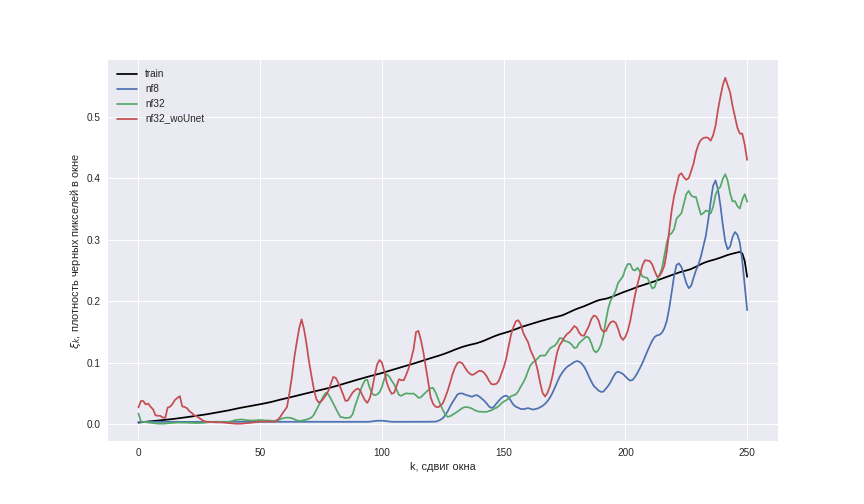
\includegraphics[width=0.95\linewidth,height=0.5\textwidth]{tr_1}}
			\caption{Плотность черных пикселей в окне в зависимости от сдвига окна}
			\label{tr-1}
		\end{figure}
		\begin{table}
			\begin{center}
				\begin{tabular}{|c|c|}
					\hline
					Сеть & Метрика \\
					\hline
					nf8 & 0.00825\\
					\hline
					nf32 & 0.00549\\
					\hline
					nf32-woUnet & 0.00688\\
					\hline
				\end{tabular}
				\caption{Значения введенной метрики для разных сетей (меньше - лучше)}
				\label{table1}
			\end{center}
		\end{table}
		\begin{figure}
			\centering{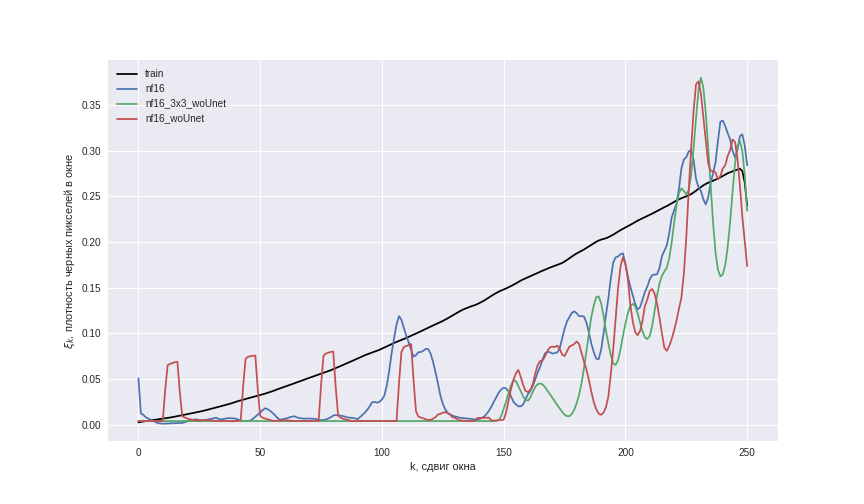
\includegraphics[width=0.95\linewidth,height=0.5\textwidth]{tr_2}}
			\caption{Плотность черных пикселей в окне в зависимости от сдвига окна}
			\label{tr-2}
		\end{figure}
		\begin{table}
			\begin{center}
				\begin{tabular}{|c|c|}
					\hline
					Сеть & Метрика \\
					\hline
					nf16 & 0.00606\\
					\hline
					nf16-woUnet & 0.00881\\
					\hline
					nf16-3x3-woUnet & 0.01034\\
					\hline
				\end{tabular}
				\caption{Значения введенной метрики для разных сетей (меньше - лучше)}
				\label{table2}
			\end{center}
		\end{table}
		\begin{figure}
			\centering{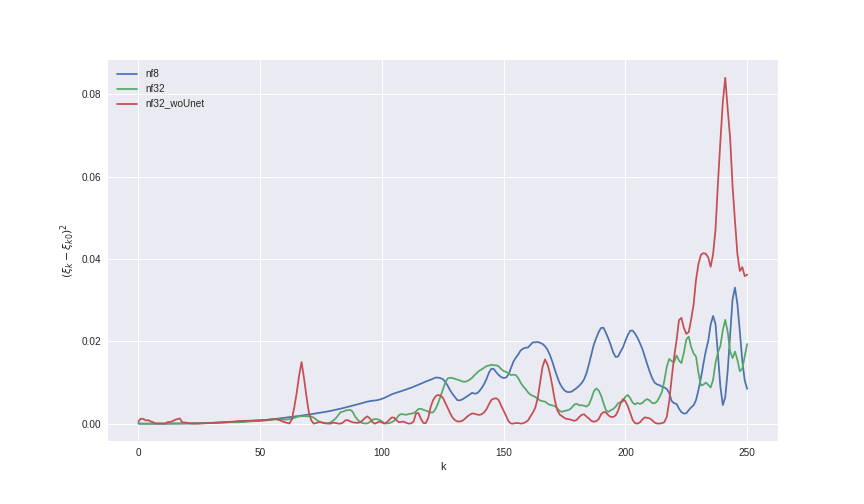
\includegraphics[width=0.95\linewidth,height=0.45\textwidth]{earr_1}}
			\caption{Квадратичное отклонение от тренда для разных сетей}
			\label{err1}
		\end{figure}
		\begin{figure}
				\centering{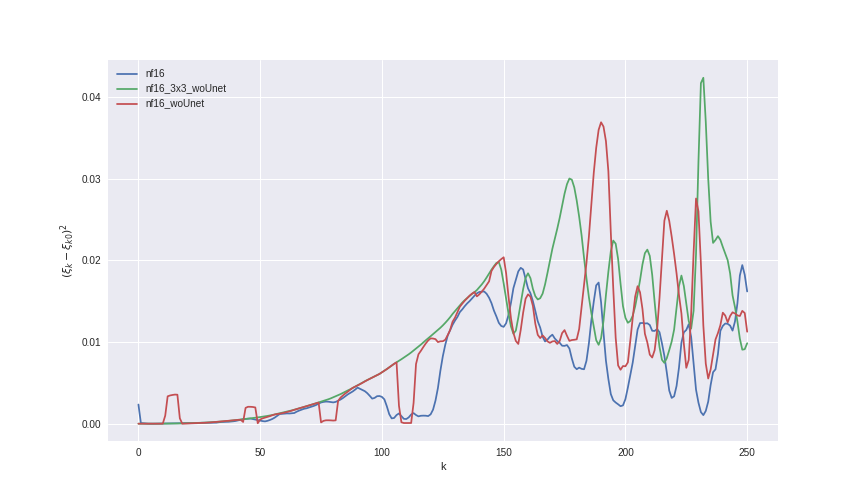
\includegraphics[width=0.95\linewidth,height=0.45\textwidth]{earr_2}}
				\caption{Квадратичное отклонение от тренда для разных сетей}
				\label{err2}
		\end{figure}
	\newpage
	\section{Выводы}
		В работе было:
		\begin{itemize}
			\item Исследовано применение архитектуры GAN для синтеза текстур с трендами
			\item Получены результаты синтеза при нескольких наборах гиперпараметров сети
			\item Проведено измерение качества генерации для каждого из наборов, используя введенную метрику
		\end{itemize}
	\section{Заключение}
		Полученные результаты показывают, что в принципе нейросеть способна уловить тренд и воспроизвести его, однако на данный момент качество генерации относительно невысоко. Необходимо провести дальнешее исследование оптимальных гиперпараметров, и, возможно, увеличить объем обучающей выборки. Также можно провести аналогичные эксперименты с другими архитектурами генераторов.
	\begin{thebibliography}{99}
		\bibitem{Voron-ML}  Воронцов К. В., "Математические методы обучения по прецедентам (теория обучения машин)".
		\bibitem{GAN} Ian J. Goodfellow, Jean Pouget-Abadie, Mehdi Mirza, Bign Xu, David Warde-Farley, Sherjil Ozair, Aaron Courville, Yoshua Bengio, "Generative Adversarial Nets" // arXiv: 1406.2661 [stat.ML], 2014
		\bibitem{GAN-2} Goodfellow, Ian, et al. "Generative adversarial nets. Advances in neural information processing systems". 2014
		\bibitem{p2p} Pedro Costa, Adrian Galdran, Maria Inês Meyer, Michael David Abràmoff, Meindert Niemeijer, Ana Maria Mendonça, Aurélio Campilho, "Towards Adversarial Retinal Image Synthesis" // arXiv: 1701.08974 [cs.CV], 2017
		\bibitem{Bishop} Christopher M. Bishop, "Pattern Recognition and Machine Learning". Springer Science+Business Media, 2006.
	\end{thebibliography}
\end{document}